% surface integral

\newpage

\begin{center}
\noindent
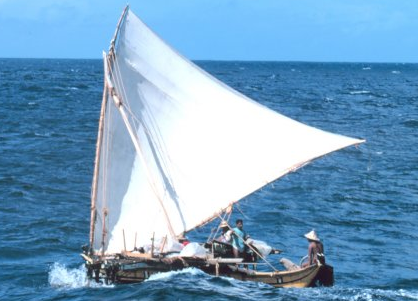
\includegraphics[scale=0.5]{sailboat.png}
\end{center}

\bigskip
\noindent
A surface integral is like adding up all the wind on a sail.
In other words, we want to compute
$$\int\!\!\!\int{\bf F\cdot n}\,da$$
where ${\bf F\cdot n}$ is the amount of wind normal to a tiny rectangle $da$.
The integral sums over the entire area of the sail.
Let $S$ be the surface of the sail parameterized by $x$ and $y$.
(In this model, the $z$ direction points downwind.)
By the properties of the cross product we have the following for the unit normal $\bf n$
and for $da$.
$${\bf n}={ {{\partial S\over\partial x}\times{\partial S\over\partial y}}\over
 {\left|{\partial S\over\partial x}\times{\partial S\over\partial y}\right|}}\qquad
da=\left|{\partial S\over\partial x}\times{\partial S\over\partial y}\right|\,dx\,dy$$
Hence
$$\int\!\!\!\int{\bf F\cdot n}\,da=\int\!\!\!\int{\bf F}\cdot
\left({{\partial S\over\partial x}\times{\partial S\over\partial y}}\right)\,dx\,dy$$

\newpage

\noindent
Evaluate the surface integral
$$\int\!\!\!\int_S{\bf F\cdot n}\,d\sigma$$
where ${\bf F}=xy^2z{\bf i}-2x^3{\bf j}+yz^2{\bf k}$, $S$ is the surface
$z=1-x^2-y^2$, $x^2+y^2\le1$ and $\bf n$ is upper.\footnote{
Kaplan, {\it Advanced Calculus,} p. 313.}

\medskip
\noindent
Note that the surface intersects the $xy$ plane in a circle.
By the right hand rule, crossing $x$ into $y$ yields $\bf n$ pointing upwards hence
$${\bf n}\,d\sigma=\left({{\partial S\over\partial x}\times{\partial S\over\partial y}}\right)\,dx\,dy$$
The following Eigenmath code computes the surface integral.
The symbols $f$ and $h$ are used as temporary variables.

\medskip
\verb$z=1-x^2-y^2$

\verb$F=(x*y^2*z,-2*x^3,y*z^2)$

\verb$S=(x,y,z)$

\verb$f=dot(F,cross(d(S,x),d(S,y)))$

\verb$h=sqrt(1-x^2)$

\verb$defint(f,y,-h,h,x,-1,1)$

$${1\over48}\pi$$

